
\section{Identification of wave spectrum model} \label{sec:part2}

\subsection{Power Spectral Density estimate}
In this subsection we want to find the Power Spectral Density (PSD) of the wave,$\psi_w$, $S_{\psi_w}(\omega)$
\newline
To calculate the PSD the matlabfunction pwelch was used. This finction returns the PSD estimate, pxx, of the input in the given the column of 
Sample Frequency = 10 Hz. Window = 4096. $\psi_w[deg]$. $[P_{xx} , f] = $\texttt{pwelch}($x_2$, window, noverlap, nfft, fs). Since the fs is given in Hz. Må konvergere $P_{xx}$ must be multiplied with $\frac{1}{2\pi}$ to get [s/rad], and f is multiplied by $2\pi$ to get [rad/s].
\newline

MATLAB, plots, grafer og kode.

\subsection{Analytic expression for transfer function and PSD}
Oppg: Find an analytic expression for the transfer function of the wave response model (from $w_w$ to $\psi_w$). Also find an analytic expression for the Power Spectral Density function of $\psi_w$, that is $P_{\psi_w}(\omega)$.

Using the same techniques as earlier to find the transfer function from $w_w$ to $\psi_w$ using \cref{eq:xidot_def} 
\begin{equation*}
    \xi_w(s) = \frac{\psi_w(s)}{s}
\end{equation*}
with $\xi_w(0) = 0$, inserting into \cref{eq:psidot_m} and using some algebra skills, we get
\begin{equation} 
    H(s) =  \frac{\psi_{w}(s)}{w_{w}(s)} = \frac{s K_w}{s^2 + 2\lambda w_w s + \omega_0^2}
\end{equation}
\bigskip

Power Spectral Density of $\psi_w \rightarrow P_{\psi_w}(\omega)$. Using Fourier transform. Know that white noise have zero-mean. Random process r(t) 

\begin{equation}
\begin{split}
    P_{\psi_w}(\omega) &= |\hat{H}(j\omega)|^2 S_w(\omega) \\
    &= \hat{H}(j\omega) \hat{H}(-j\omega) S_{\psi_w}(\omega)
\end{split}
\end{equation}
where $S_w(j\omega) = 0$ 
\newline

\begin{equation}
\begin{split}
    H(j\omega)H(-j\omega) &= \frac{j\omega K_w}{(j\omega)^2 + 2\lambda w_0 j\omega + \omega_0^2}*\frac{-j \omega K_w}{(-j\omega)^2 - 2\lambda w_0 j\omega + \omega_0^2} \\
    &= \frac{(\omega K_w)^2}{\omega^4 - 2\omega^2 \omega_0^2 + 4 \lambda^2 \omega_0^2 \omega^2 + \omega_0^4}
\end{split}
\end{equation} 

White noise is only theoretic. You cannot get something that has infinite variance. 
\begin{equation*}
    S_w(\omega) = \mathbb{F} \{R_w(\tau)^2\} = 1 \ , \ R_w = \delta(\tau) \sigma^2 = \delta(t)
\end{equation*} \todo{skal noen av disse være fancy krøllegreier}

Er P og S av psi den samme funksjonen eller er P den analytiske og S den estimerte??





\subsection{Resonance frequency from estimated PSD} \label{sec:5.2.c}
Oppg: Find $\omega_w$ from the estimated $S_{\psi_w}(\omega)$ in part a).
\newline
$\omega_0$ is the maximum of the power spectral density function, $S_{\psi_w}(\omega)$, which gives
\begin{equation}
    \omega_0 = 0.7823
\end{equation}

\begin{figure}[H]
    \centering
    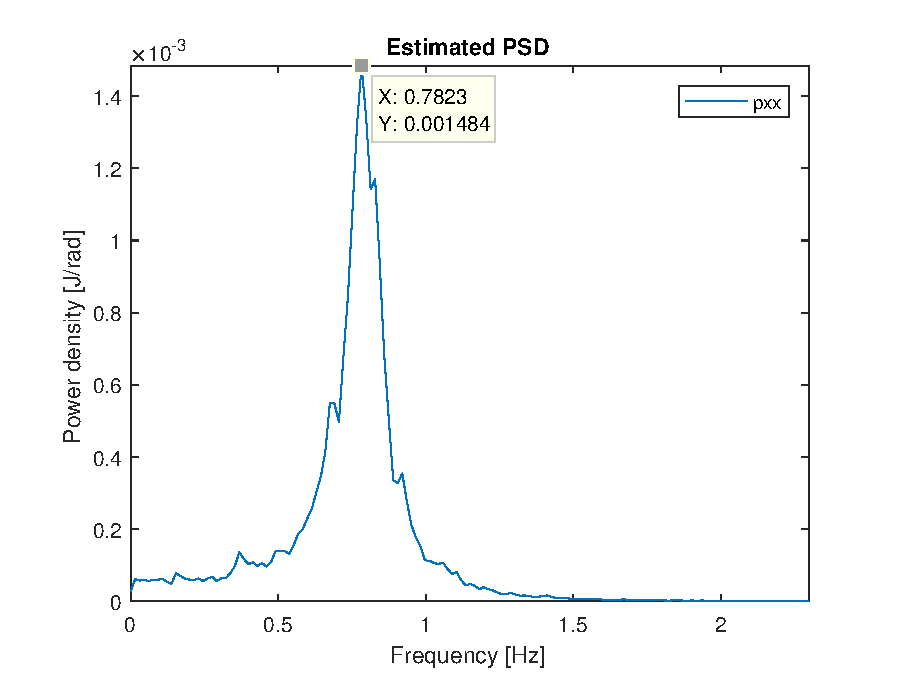
\includegraphics[width=0.5\linewidth]{Part2_pics/p2c_omega0.eps}
    \caption{Reading off $\omega_0$ from the estimated PSD found in 5.2.a}
    \label{fig:p2c}
\end{figure}

\subsection{Damping factor $\lambda$} \label{sec:5.2.d}
Oppg: To have a complete model for the wave response we need to identify the damping factor $\lambda$. Define $K_w = 2 \lambda \omega_0 \sigma$ where $\sigma^2$ is the peak value of $P_{\psi_w}(\omega)$. Find $\lambda$ by fitting the $P_{\psi_w}(\omega)$ to the estimate of the PSD, $S_{\psi_w}(\omega)$. Use trial and error. Alternatively, you may use curve-fitting methods in MATLAB (Hint: \texttt{doc lsqcurvefit}). Include plot for comparison manner.
\newline

Know that $K_w = \lambda \omega_0 \sigma$ where $\sigma^2$ is the peak value of $P_{\psi_w}(\omega)$. From looking at PLOTS from \cref{sec:5.2.c} we see that $y = 0.001482$. 

Use the transferfunction for ??. After some trial and error we choose $\lambda$ to be 0.8 or 0.7.

\begin{figure}[H]
\begin{subfigure}{0.5\textwidth}
    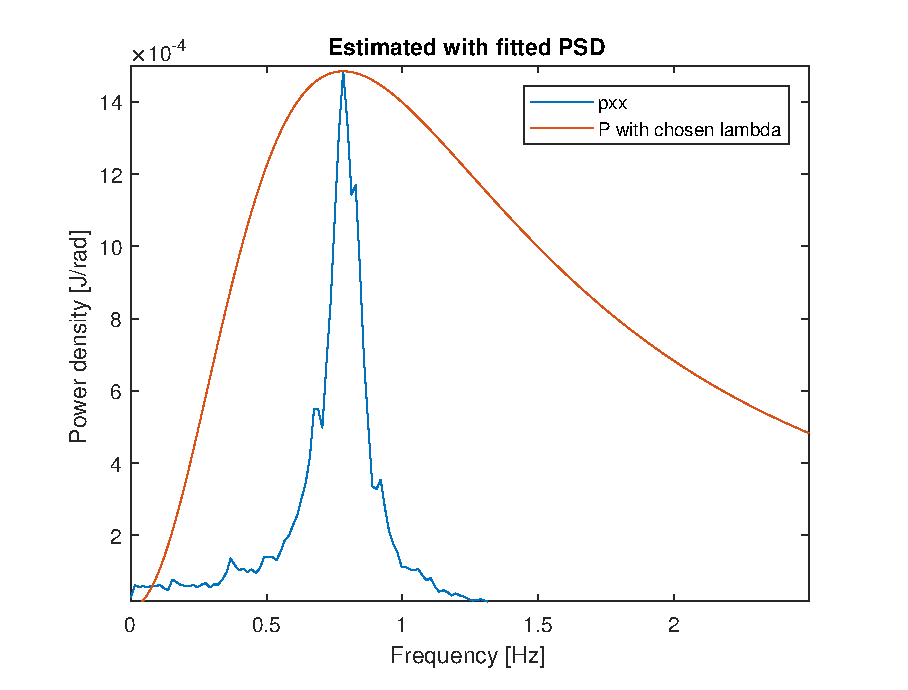
\includegraphics[width=1\linewidth]{Part2_pics/p2d_lambda_1.eps}
    \caption{$\lambda = 1$}
\end{subfigure}
\begin{subfigure}{0.5\textwidth}
    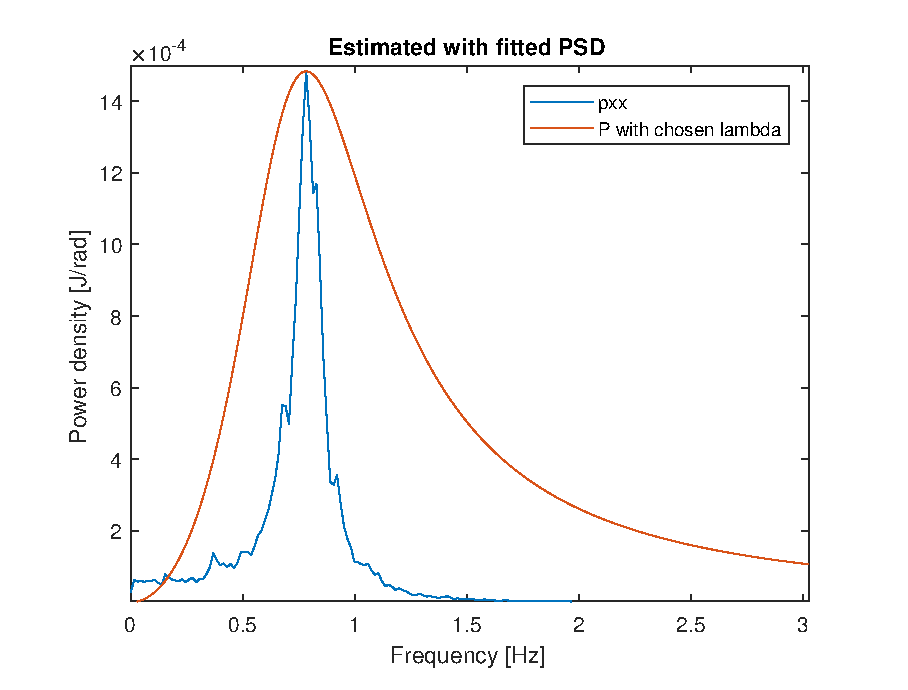
\includegraphics[width=1\linewidth]{Part2_pics/p2d_lambda_05.eps}
    \caption{$\lambda = 0.5$}
\end{subfigure}
\caption{To large values for $\lambda$}
\label{fig:p2d1}
\end{figure}

\begin{figure}[H]
\begin{subfigure}{0.5\textwidth}
    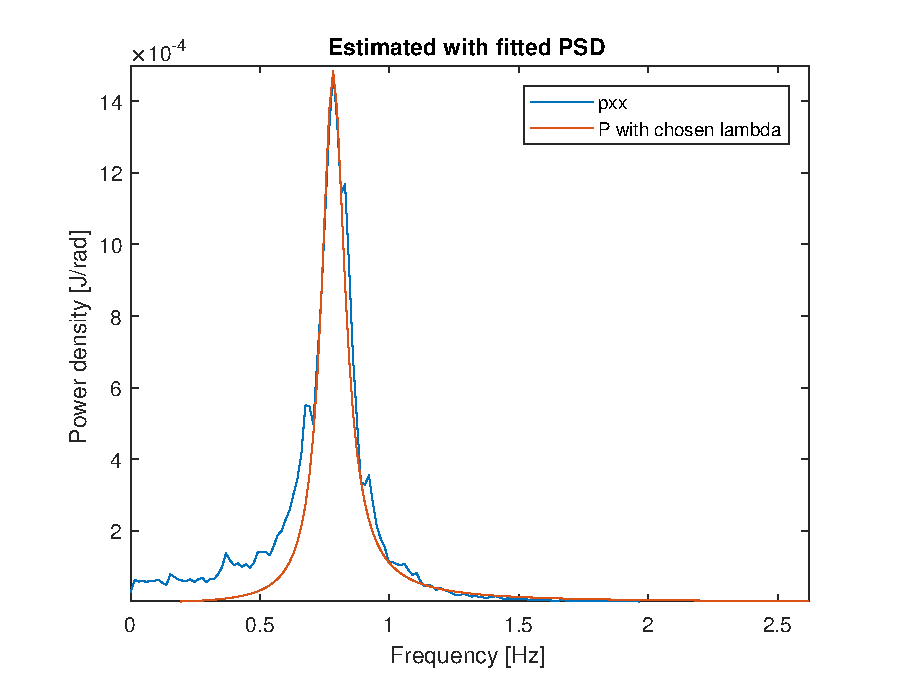
\includegraphics[width=1\linewidth]{Part2_pics/p2d_lambda_007.eps}
    \caption{$\lambda = 0.07$}
\end{subfigure}
\begin{subfigure}{0.5\textwidth}
    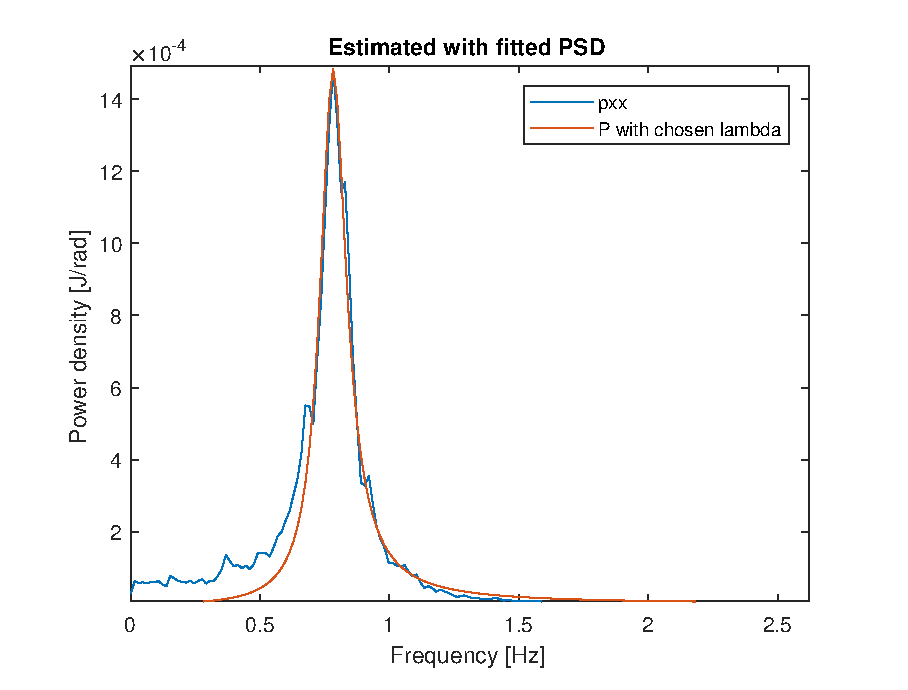
\includegraphics[width=1\linewidth]{Part2_pics/p2d_lambda_008.eps}
    \caption{$\Lambda = 0.08$}
\end{subfigure}
\caption{The best found values for $\lambda$}
\label{fig:p2d2}
\end{figure}